\newpage
\chapter{SPARTA}

SPARTA is an acronym for Stochastic PArallel Rarefied-gas Time-accurate Analyzer. SPARTA was developed by Sandia National Laboratories under the US Department of Energy. The chief authors of SPARTA are Michael Gallis, Steve Plimpton, and Stan Moore. Plimpton et al. (2019) describe how SPARTA functions in their work on implementing DSMC on petaflop supercomputers \cite{plimpton2019direct}. \\

\no SPARTA is a parallel DSMC code for performing simulations of low-density gases in 2D or 3D. Particles advect through a hierarchical Cartesian grid that overlays the simulation box. The grid is used to group particles by grid cell for purposes of performing collisions and chemistry. Physical objects with triangulated surfaces can be embedded in the grid, creating cut and split grid cells. The grid is also used to efficiently find particle/surface collisions. Since the fundamental DSMC algorithm is inherently parallel, the challenge is not to parallelize the code but to balance computations across a large number of processors. \\

\no SPARTA has three kinds of data : particles, grid cells, and optionally surface elements. The grid used by SPARTA is a rectilinear hierarchical grid \textit{i.e.,} each grid cell can have more grid cells within itself, recursively. All these child grid cells are also cuboidal in shape. Figure \ref{img:grid} was taken from \cite{plimpton2019direct} and represents the hierarchical grid around the Apollo space capsule.

\begin{figure}[H]
  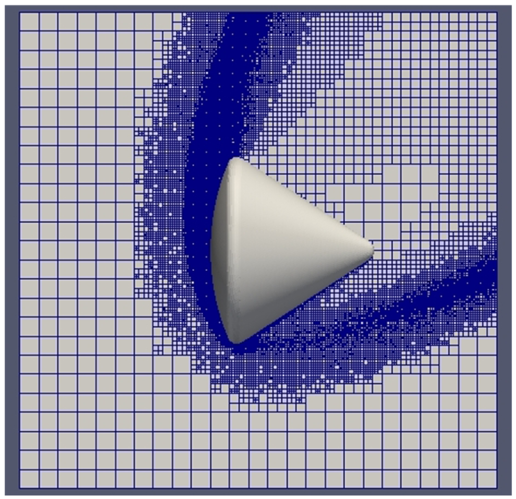
\includegraphics[scale=0.5]{Pictures/Chapter_4_SPARTA/Grid.png}
  \centering
  \caption{A 2D slice of a 3D hierarchical grid around the Apollo space capsule [Source : \cite{plimpton2019direct}]}
  \label{img:grid}
\end{figure}

\no SPARTA has the ability to run parallely by assigning certain grid cells to certain processors. An example is given in Figure \ref{img:parallel} which was taken from \cite{plimpton2019direct} where each color represents a particular processor.

\begin{figure}[H]
  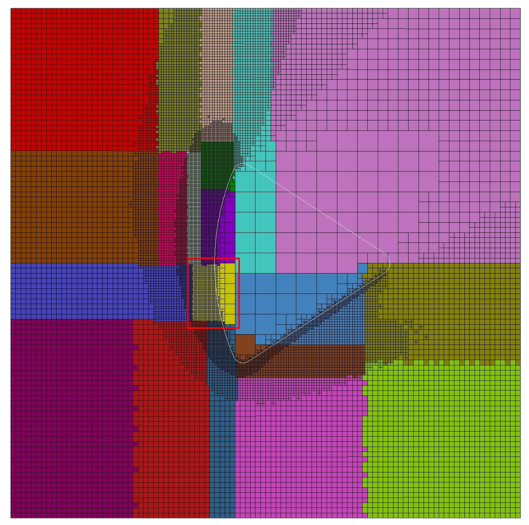
\includegraphics[scale=0.5]{Pictures/Chapter_4_SPARTA/Parallel.png}
  \centering
  \caption{A 5-level 2D hierarchical grid around the Apollo space capsule [Source : \cite{plimpton2019direct}]}
  \label{img:parallel}
\end{figure}

\no There have been several bench-marking problems to show that SPARTA indeed does provide physically accurate solutions and some of them will be discussed subsequently.

\section{Effect of Slip on Vortex Shedding}

This study was done by Gallis and Torczynski \cite{gallis2021effect} to analyse the effect of slip on the vortex shedding in a flow around a circular cylinder. Typically most studies assume that the no-slip condition applies on the cylinder surface. They perform their simulations at a Reynolds number of 100, a Mach number of 0.3 and a corresponding Knudsen number of 0.0048. The simulation domain is described in Figure \ref{img:sim} taken from \cite{gallis2021effect}.

\begin{figure}[H]
  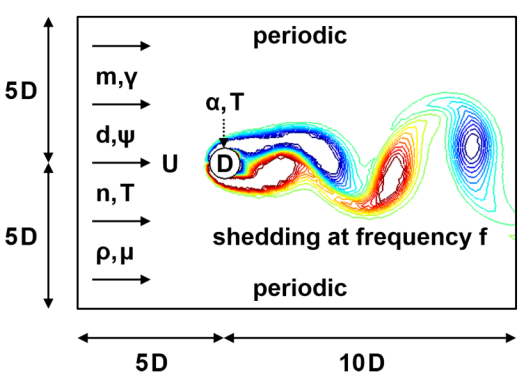
\includegraphics[scale=0.5]{Pictures/Chapter_4_SPARTA/Sim.png}
  \centering
  \caption{Simulation domain [Source : \cite{gallis2021effect}]}
  \label{img:sim}
\end{figure}

\no The cylinder diameter $D$ was chosen to be 1 m for convenience. The gas was assumed to be Argon-like with a molecular mass of $m = 66.3 \times 10^{-27} kg$, specfic heat ratio $\gamma = 5/3$, viscosity $\mu = 2.117 \times 10^{-5} Pa \: s$ at temperature $T = 273.15K$. For the non-dimensional numbers described above,  the freestream velocity, density, number density and molecular mean free path are $U = 92.37 m/s, \: \rho = 2.292 \times 10^{-5} kg/m^3, \: n = 3.457 \times 10^{20} 1/m^3$ and $\lambda = 0.0048m$. The grid cell size is chosen to be about one-fourth the mean free path and the time step is chosen to be about one-fourth of the mean collision time. There are about 100 particles per grid cell, totaling about 8 billion particles. The cylinder's surface reflects diffusively with a probability $\alpha$ and specularly with a probability $1 - \alpha$ where $\alpha$ is the \textbf{accommodation coefficient}.

\no The same simulation was also performed using CFD on COMSOL Multiphysics and the results were compared. Figure \ref{gra:comp} was taken from their work \cite{gallus2021effect} and highlights that the results are largely in agreement with each other, with DSMC being a little bit more noisy than CFD due to its statistical nature.

\begin{figure}[H]
  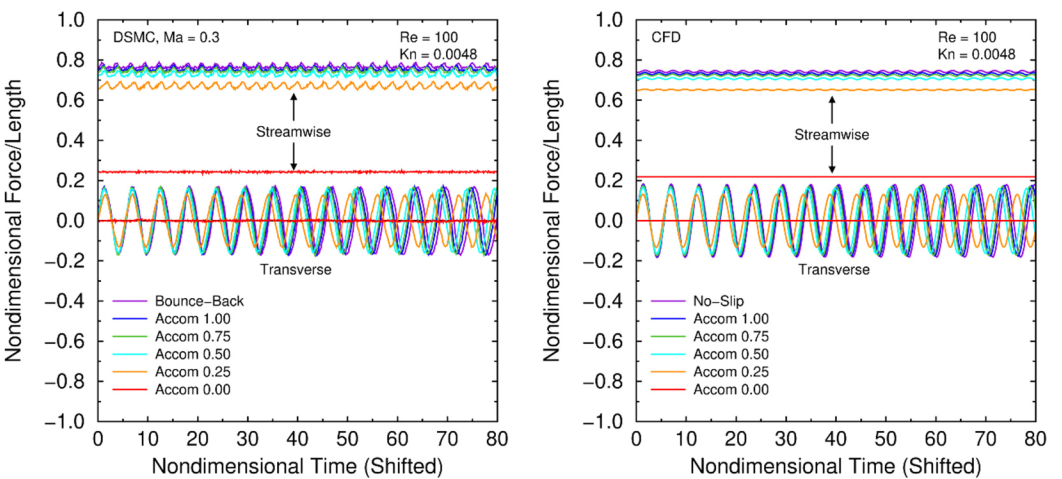
\includegraphics[scale=0.4]{Pictures/Chapter_4_SPARTA/Comp.png}
  \centering
  \caption{DMSC (left) and CFD (right) force histories at late times with periodic vortex shedding [Source : \cite{gallis2021effect}]}
  \label{img:comp}
\end{figure}

\no Clearly, the CFD and DSMC simulations are in good agreement, indicating that the DSMC method is physically accurate. However, for low Mach number (and consequently low Knudsen numbers), CFD is a lot more computationally efficient as simulating particle collisions under these conditions is extreme. Almost all the physical phenomena can be captured by conventional mathematical models like the Navier-Stokes equations. \\

\no In the upcoming chapters, some of my own simulations using SPARTA and their results will be discussed.